\documentclass{beamer}

\pdfmapfile{+sansmathaccent.map}


\mode<presentation>
{
  \usetheme{Warsaw} % or try Darmstadt, Madrid, Warsaw, Rochester, CambridgeUS, ...
  \usecolortheme{seahorse} % or try seahorse, beaver, crane, wolverine, ...
  \usefonttheme{serif}  % or try serif, structurebold, ...
  \setbeamertemplate{navigation symbols}{}
  \setbeamertemplate{caption}[numbered]
} 


%%%%%%%%%%%%%%%%%%%%%%%%%%%%
% itemize settings

\definecolor{mypink}{RGB}{255, 30, 80}
\definecolor{mydarkblue}{RGB}{60, 160, 255}
\definecolor{myblue}{RGB}{240, 240, 255}
\definecolor{mygreen}{RGB}{0, 200, 0}
\definecolor{mygreen2}{RGB}{245, 255, 230}
\definecolor{mygray}{gray}{0.8}

\setbeamertemplate{itemize items}[default]

\setbeamertemplate{itemize item}{\color{mygreen}$\blacksquare$}
\setbeamertemplate{itemize subitem}{\color{mydarkblue}$\blacktriangleright$}
\setbeamertemplate{itemize subsubitem}{\color{mygray}$\blacksquare$}



\setbeamercolor{palette quaternary}{fg=white,bg=mydarkblue}
\setbeamercolor{titlelike}{parent=palette quaternary}

\setbeamercolor{palette quaternary2}{fg=black,bg=myblue}
\setbeamercolor{frametitle}{parent=palette quaternary2}



\setbeamerfont{frametitle}{size=\Large,series=\scshape}
\setbeamerfont{framesubtitle}{size=\normalsize,series=\upshape}





%%%%%%%%%%%%%%%%%%%%%%%%%%%%
% block settings

\setbeamercolor{block title}{bg=red!30,fg=black}

\setbeamercolor*{block title example}{bg=mygreen!40!white,fg=black}

\setbeamercolor*{block body example}{fg= black,
bg= mygreen2}


%%%%%%%%%%%%%%%%%%%%%%%%%%%%
% URL settings
\hypersetup{
    colorlinks=true,
    linkcolor=blue,
    filecolor=blue,      
    urlcolor=blue,
}

%%%%%%%%%%%%%%%%%%%%%%%%%%

\renewcommand{\familydefault}{\rmdefault}

\usepackage{amsmath}
\usepackage{mathtools}


\usepackage{subcaption}


\DeclareMathOperator*{\argmin}{arg\,min}
\newcommand{\bo}[1] {\mathbf{#1}}


%%%%%%%%%%%%%%%%%%%%%%%%%%%%
% code settings

\usepackage{listings}
\usepackage{color}
% \definecolor{mygreen}{rgb}{0,0.6,0}
% \definecolor{mygray}{rgb}{0.5,0.5,0.5}
\definecolor{mymauve}{rgb}{0.58,0,0.82}
\lstset{ 
  backgroundcolor=\color{white},   % choose the background color; you must add \usepackage{color} or \usepackage{xcolor}; should come as last argument
  basicstyle=\footnotesize,        % the size of the fonts that are used for the code
  breakatwhitespace=false,         % sets if automatic breaks should only happen at whitespace
  breaklines=true,                 % sets automatic line breaking
  captionpos=b,                    % sets the caption-position to bottom
  commentstyle=\color{mygreen},    % comment style
  deletekeywords={...},            % if you want to delete keywords from the given language
  escapeinside={\%*}{*)},          % if you want to add LaTeX within your code
  extendedchars=true,              % lets you use non-ASCII characters; for 8-bits encodings only, does not work with UTF-8
  firstnumber=0000,                % start line enumeration with line 0000
  frame=single,	                   % adds a frame around the code
  keepspaces=true,                 % keeps spaces in text, useful for keeping indentation of code (possibly needs columns=flexible)
  keywordstyle=\color{blue},       % keyword style
  language=Octave,                 % the language of the code
  morekeywords={*,...},            % if you want to add more keywords to the set
  numbers=left,                    % where to put the line-numbers; possible values are (none, left, right)
  numbersep=5pt,                   % how far the line-numbers are from the code
  numberstyle=\tiny\color{mygray}, % the style that is used for the line-numbers
  rulecolor=\color{black},         % if not set, the frame-color may be changed on line-breaks within not-black text (e.g. comments (green here))
  showspaces=false,                % show spaces everywhere adding particular underscores; it overrides 'showstringspaces'
  showstringspaces=false,          % underline spaces within strings only
  showtabs=false,                  % show tabs within strings adding particular underscores
  stepnumber=2,                    % the step between two line-numbers. If it's 1, each line will be numbered
  stringstyle=\color{mymauve},     % string literal style
  tabsize=2,	                   % sets default tabsize to 2 spaces
  title=\lstname                   % show the filename of files included with \lstinputlisting; also try caption instead of title
}

%%%%%%%%%%%%%%%%%%%%%%%%%%%%
% tikz settings

\usepackage{tikz}
\tikzset{every picture/.style={line width=0.75pt}}


\title{Stability}
\subtitle{Control Theory, Lecture 2}
\author{by Sergei Savin}
\centering
\date{Spring 2021}



\begin{document}
\maketitle


\begin{frame}{Content}

\begin{itemize}
% \item Motivation
% \item Ordinary differential equations
%     \begin{itemize}
%     \item 1st order
%     \item n-th order
%     \end{itemize}
% \item Linear differential equations
%     \begin{itemize}
%     \item 1st order
%     \item n-th order
%     \item ...are what we will study
%     \end{itemize}
% \item Changing n-th order ODE to a State-Space form
\item Read more
\end{itemize}

\end{frame}



\begin{frame}{Critical point (node)}
% \framesubtitle{O}
\begin{flushleft}

Consider the following ODE:

\begin{equation}
    \dot{\bo{x}} = \bo{f} (\bo{x}, t)
\end{equation}

Let $\bo{x}_0$ be such a state that:

\begin{equation}
    \bo{f} (\bo{x}_0, t) = 0
\end{equation}

Then such state $\bo{x}_0$ is called a \emph{node} or a \emph{critical point}.

\end{flushleft}
\end{frame}



\begin{frame}{Stability}
% \framesubtitle{O}
\begin{flushleft}

Node $\bo{x}_0$ is called \emph{stable} iff for any constant $\delta$ there exists constant $\varepsilon$ such that:

\begin{equation}
    ||\bo{x}(0) - \bo{x}_0|| < \delta \ \longrightarrow \ ||\bo{x}(t) - \bo{x}_0|| < \varepsilon
\end{equation}

\bigskip

Think of it as "for any initial point that lies at most $\delta$ away from $\bo{x}_0$, the rest of the trajectory $\bo{x}(t)$ will be at most $\varepsilon$ away from $\bo{x}_0$".

\bigskip

Or, more picturesque, think of it as "the solutions with different initial conditions do not diverge from the node"

\end{flushleft}
\end{frame}


\begin{frame}{Asymptotic stability}
% \framesubtitle{O}
\begin{flushleft}

Node $\bo{x}_0$ is called \emph{asymptotically stable} iff for any constant $\delta$ it is true that:

\begin{equation}
    ||\bo{x}(0) - \bo{x}_0|| < \delta \ \longrightarrow \ 
    \lim_{t\to\infty} \bo{x}(t) = \bo{x}_0
\end{equation}

\bigskip

Think of it as "for any initial point that lies at most $\delta$ away from $\bo{x}_0$, the trajectory $\bo{x}(t)$ will asymptotically approach the point $\bo{x}_0$".

\bigskip

Or, more picturesque, think of it as "the solutions with different initial conditions converge to the node"

\end{flushleft}
\end{frame}




\begin{frame}{Stability vs Asymptotic stability}
% \framesubtitle{O}
\begin{flushleft}

\begin{example}
Consider dynamical system $\dot{x} = 0$, and solution $x = 7$. This solution is stable, but not asymptotically stable (other solutions do not diverge from $x = 7$, but do not converge to it either).
\end{example}

\begin{example}
Consider dynamical system $\dot{x} = -x$, and solution $x = 0$. This solution is stable and asymptotically stable (other solutions converge to $x = 0$).
\end{example}

\begin{example}
Consider dynamical system $\dot{x} = x$, and solution $x = 0$. This solution is unstable (other solutions diverge from $x = 0$).
\end{example}

\end{flushleft}
\end{frame}



\begin{frame}{LTI and autonomous LTI}
% \framesubtitle{O}
\begin{flushleft}

Consider the following linear ODE:

\begin{equation}
    \dot{\bo{x}} = \bo{A} \bo{x} + \bo{B} \bo{u}
\end{equation}

This is called a \emph{linear time-invariant system}, or \emph{LTI}.

\bigskip

Consider the following linear ODE:

\begin{equation}
    \dot{\bo{x}} = \bo{A} \bo{x}
\end{equation}

This is also an LTI, but it is also called an \emph{autonomous system}, since its evolution depends only on the state of the system.

\end{flushleft}
\end{frame}




\begin{frame}{Stability of autonomous LTI}
\framesubtitle{Example: real eigenvalues}
\begin{flushleft}

Consider autonomous LTI:

\begin{equation}
    \dot{\bo{x}} = \bo{A} \bo{x}
\end{equation}

where $\bo{A}$ can be decomposed via eigen-decomposition as $\bo{A} = \bo{V} \bo{D} \bo{V}^{-1}$, where $\bo{D}$ is a diagonal matrix. 

\bigskip

\begin{equation}
    \dot{\bo{x}} = \bo{V} \bo{D} \bo{V}^{-1} \bo{x}
\end{equation}

Multiply it by $\bo{V}^{-1} 
\ \longrightarrow \ 
\bo{V}^{-1} \dot{\bo{x}} = \bo{V}^{-1} \bo{V} \bo{D} \bo{V}^{-1} \bo{x}$.

Define $\bo{z} = \bo{V}^{-1} \bo{x} 
\ \longrightarrow \
\dot{\bo{z}} = \bo{D} \bo{z}$.

\bigskip

Since elements of $\bo{D}$ are real, we can clearly see, that iff they are \emph{all negative} will the system be asymptotically stable. If they are non-positive, the system is stable. And those elements are eigenvalues of $\bo{A}$.

\end{flushleft}
\end{frame}



\begin{frame}{Stability of autonomous LTI}
\framesubtitle{Example: complex eigenvalues, part 1}
\begin{flushleft}

Assume that $\bo{A}$ can be decomposed via eigen-decomposition as $\bo{A} = \bo{U} \bo{C} \bo{U}^{-1}$, where $\bo{C}$ is a complex-valued diagonal matrix and $\bo{U}$ is a complex-valued inevitable matrix. 

\bigskip

We can perform the same steps (multiply by $\bo{U}^{-1}$, then define $\bo{z} = \bo{U}^{-1} \bo{x}$) to arrive at:

\begin{equation}
    \dot{\bo{z}} = \bo{C} \bo{z}
\end{equation}

which falls into a set of independent equations, with complex coefficients $c_i$:

\begin{equation}
    \dot{z}_i = c_i z_i
\end{equation}

The solution is:

\begin{equation}
    z_i = k_0 e^{c_i t}
\end{equation}

\end{flushleft}
\end{frame}



\begin{frame}{Stability of autonomous LTI}
\framesubtitle{Example: complex eigenvalues, part 2}
\begin{flushleft}

The solution $z_i = k_0 e^{c_i t}$, where $c_i = \alpha_i + i \beta_i$, can be decomposed using Euler's identity:

\[
    z_i = k_0 e^{c_i t} =
    k_0 e^{(\alpha_i + i \beta_i) t} =
    k_0 e^{\alpha_i t} 
          e^{i \beta_i t} = 
    k_0 e^{\alpha_i t} 
    (\cos(\beta_i t) + i \sin(\beta_i t))
\]

As you can see, brackets $(\cos(\beta_i t) + i \sin(\beta_i t))$ has a constant norm, $|| (\cos(\beta_i t) + i \sin(\beta_i t)) || = 1$. Therefore, norm of $z_i$ depends entirely on the norm of $e^{\alpha_i t}$, which is:

\begin{enumerate}
    \item constant if $\alpha_i = 0$, hence the system is stable. 
    \item decreasing if $\alpha_i < 0$, hence the system is asymptotically stable. 
    \item increasing if $\alpha_i > 0$, hence the system is unstable. 
\end{enumerate}



\end{flushleft}
\end{frame}




\begin{frame}{Stability of autonomous LTI}
\framesubtitle{General case}
\begin{flushleft}

Consider an autonomous LTI:

\begin{equation}
\label{eq:LTI}
    \dot{\bo{x}} = \bo{A} \bo{x}
\end{equation}

\begin{definition}
Eq. \eqref{eq:LTI} is stable iff real parts of eigenvalues of $\bo{A}$ are non-positive.
\end{definition}

\begin{definition}
Eq. \eqref{eq:LTI} is asymptotically stable iff real parts of eigenvalues of $\bo{A}$ are negative.
\end{definition}

\end{flushleft}
\end{frame}




\begin{frame}{Stability of autonomous LTI}
\framesubtitle{Illustration}
\begin{flushleft}

Here is an illustration of \emph{phase portraits} of two-dimensional LTIs with different types of stability:

\begin{figure}
    \centering
    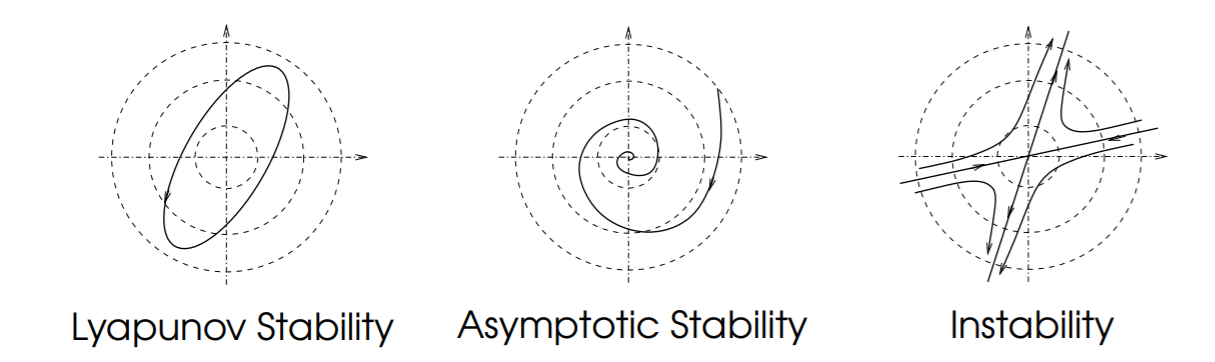
\includegraphics[width=1.0\linewidth]{Stability.PNG}
    \caption{phase portraits for different types of stability}
    \label{fig:Stability}
\end{figure}

\bigskip

\scriptsize{Credit: \href{http://staff.uz.zgora.pl/wpaszke/materialy/spc/Lec13.pdf}{staff.uz.zgora.pl/wpaszke/materialy/spc/Lec13.pdf}}

\end{flushleft}
\end{frame}






\begin{frame}{Read more}

\begin{itemize}
\item Control Systems Design, by Julio H. Braslavsky \href{http://staff.uz.zgora.pl/wpaszke/materialy/spc/Lec13.pdf}{staff.uz.zgora.pl/wpaszke/materialy/spc/Lec13.pdf}


\end{itemize}

\end{frame}



\begin{frame}{Thank you!}
\centerline{Lecture slides are available via Moodle.}
\bigskip
\centerline{You can help improve these slides at:}
\centerline{\href{https://github.com/SergeiSa/Control-Theory-Slides-Spring-2021}{github.com/SergeiSa/Control-Theory-Slides-Spring-2021}}
\bigskip
\centerline{Check Moodle for additional links, videos, textbook suggestions.}
\end{frame}

\end{document}
